% !TEX root = ../Sesiones-TDA-Ejercicios.tex



\chapter{Listas}

\etocsetnexttocdepth{3}
\etocsettocstyle{\hrule \vskip 0.15cm \subsubsection*{Índice Parcial}\vskip -0.65cm}{\vskip 0.15cm\hrule}
\localtableofcontents

\

\

\centerline{\Large \bf Teoría}

\formatoNormal



\



%%%%%%%%%%%%%%%%%%%%%%%%%%%%%%%%%%%%%%%%%%%%%%%%%%%%%%%%%%%%%%%%%%%%%%%%%%%%%%%%%%%%
%%%%%%%%%%%%%%%%%%%%%%%%%%%%%%%%%%%%%%%%%%%%%%%%%%%%%%%%%%%%%%%%%%%%%%%%%%%%%%%%%%%%

\section*{4.A TDAs Lineales}
\addcontentsline{toc}{section}{4.A. TDAs Lineales}


Son aquellos que se pueden expresar como una sucesión finita de elementos $a_1, a_2,\ldots, a_n$. Aunque cada TDA tiene sus propias operaciones, las más importantes son:
\begin{itemize}
\item Agregar un elemento a la sucesión.
\item Eliminar un elemento de la sucesión.
\item Consultar un elemento de la sucesión. 
\end{itemize}


Destacan los TDAs con ordenación lineal que son aquellos donde cada objeto tiene exactamente un predecesor inmediato o un sucesor inmediato. Destacan el primer objeto (que no tiene predecesor) y el último objeto (que no tiene sucesor). Matemáticamente,

Una relación binaria $a\preceq b$ ($a$ precede o es igual a $b$) entre dos objetos es una ordenación lineal sii cumple las siguientes propiedades:
\begin{description}
\item[Completa]  o total. $\forall \; a, b$, o bien $a\preceq b$ o bien $b\preceq a$,
\item[Transitiva.] si $a\preceq b$ y $b\preceq c$, esto implica que $a\preceq c$, y
\item[Antisimétrica.] Si se cumple   $a\preceq b$ y $b\preceq a$, se sigue que $a = b$
\end{description}
Diremos que $a\prec b$ ($a$ precede a $b$) sii $a\preceq b$ y $a\not = b$.

Las operaciones adicionales en este tipo de contenedor son:

\begin{itemize}
\item Acceder al k-ésimo objeto del orden. En particular, al primer o último objeto en el orden lineal,
\item Recorrer todos los objetos del contenedor en dicho orden.
\item Dado un objeto $a$ que puede, o no,  estar en el contenedor, 
	\begin{itemize}
	\item buscar el objeto predecesor o sucesor en el contenedor.
	\item contar todos los objetos que le preceden o todos los que le suceden.
	\end{itemize}
\item Inserta un nuevo objeto o reemplazar el objeto en la k-ésima posición,
\item Dada una referencia al k-ésimo objeto, inserte un nuevo objeto antes o después de ese objeto; o eliminar el objeto antes o después del k-ésimo objeto.
\end{itemize}

Algunos ejemplos de este tipo abstracto de contenedores son: string, listas, listas ordenadas, pilas, colas, colas de prioridad.

\

También se incluyen en este tipo de TDA a aquellos donde la relación entre ellos no es relevante. P.e. conjuntos abstractos o conjuntos asociativos abstractos.

Las operaciones en este tipo de contenedor son las operaciones que tiene cualquier  contenedor general:

\begin{itemize}
\item Acceder al número de objetos del contenedor,
\item Determinar si el contenedor está vacío,
\item Insertar un nuevo objeto en el contenedor,
\item Determinar si un objeto está en el contenedor (membresía),
\item Sacar un objeto del contenedor y
\item Quitar todos los datos (limpiar) del contenedor.
\end{itemize}


En la Sesión \ref{chap:secuenciasPython} ya estudió los tipos de datos integrados en Python relacionados con las secuencias. También implementó los diccionarios, conjunto y bags usando el tipo de dato \cm{list}. En esta sesión vamos a estudiar la forma generar de implementar los TDA lineales e implamentaremos algunos en particular.



%%%%%%%%%%%%%%%%%%%%%%%%%%%%%%%%%%%%%%%%%%%%%%%%%%%%%%%%%%%%%%%%%%%%%%%%%%%%%%%%%%%%
%%%%%%%%%%%%%%%%%%%%%%%%%%%%%%%%%%%%%%%%%%%%%%%%%%%%%%%%%%%%%%%%%%%%%%%%%%%%%%%%%%%%

\section*{4.B Implementación de TDAs lineales}
\addcontentsline{toc}{section}{4.B. Implementación de TDAs lineales}

Existen 3 grandes grupos de estructuras de datos para implementar los TDAs lineales:

\begin{itemize}
\item Arrays. La colección de objetos se sitúan en cada una de las posiciones del array.
\item Otras estructuras integradas del lenguaje. En Python, por ejemplo, se pueden usar la secuencia más adecuada.
\item Estructuras enlazadas. Una estructura enlazada es aquella que se construye utilizando como estructura básica una que tiene el siguiente patrón:

\hfil
\begin{minipage}{.25\textwidth}
\begin{pyverbatim}[][frame=single]
struct node {
   TD valor;
   node reference1;
   node reference2;
   ...
}
\end{pyverbatim}
\end{minipage}


Esta estructura básica, llamada también como \textbf{nodo, consta de un campo donde se almacena un valor y uno o varios campos que almacenan referencias a la misma estructura básica} (hace referencia a otros nodos del mismo tipo). 


\begin{note} \label{def:coneptoNodo}
Un nodo nos sirve para representar muchos conceptos como los elementos de una lista o los vértices de un árbol o grafo.  Además esta representación puede ser distinta incluso para representar el mismo concepto. Por ejemplo, se puede representar una lista como una lista simplemente enlazada, una lista doblemente enlazada o una lista circular. Como verá más adelante, cada una de las 3 representaciones indicadas usan una estructura de nodo, solo que cada una de las representaciones usa las referencias del nodo de forma diferente. Los nodos también se usa en técnicas de búsqueda (búsqueda en anchura, en profundidad, Dijkstra, etc). En la práctica, nos podemos encontrar con la necesidad de mezclar nodos de distintos tipos, naturaleza y propósitos. Por ejemplo, usar nodos para representar una lista y usar otros nodos para hacer una búsqueda a partir de una lista que está representada mediante nodos.

\textbf{
El concepto de nodo siempre es el mismo: \key{es una representación} que consta de valor+referencias. Cómo y para qué se va a usar condiciona al valor que almacena (o valores) y la cantidad de referencias.}
\end{note}


\end{itemize}

Uno podría argumentar que si un lenguaje de programación ya tiene implementado los TDAs para qué dedicar esfuerzos en implementarlos de nuevo. Hay dos motivos obvios por los que conviene aprender a implementarlos:
\begin{enumerate}
\item En una asignatura de programación debe conocer cómo se implementan los TDAs. Es un conocimiento básico de programación.

Es como decir que para qué aprender derivadas si ya hay programas informáticos que las calculan.

\item El TDA implementado por el lenguaje puede contener primitivas insuficientes o poco adecuadas para nuestros propósitos. 

Puede verse obligado a tener que extender la clase que los implementa o simplemente adaptarla a su necesidades. Pero esto no será posible si no conoce el punto anterior.
\end{enumerate}




%%%%%%%%%%%%%%%%%%%%%%%%%%%%%%%%%%%%%%%%%%%%%%%%%%%%%%%%%%%%%%%%%%%%%%%%%%%%%%%%%%%%
%%%%%%%%%%%%%%%%%%%%%%%%%%%%%%%%%%%%%%%%%%%%%%%%%%%%%%%%%%%%%%%%%%%%%%%%%%%%%%%%%%%%

\section*{4.C TDA Lista}
\addcontentsline{toc}{section}{4.C. TDA Lista}



%%%%%%%%%%%%%%%%%%%%%%%%%%%%%%%%%%%%
%%%%%%%%%%%%%%%%%%%%%%%%%%%%%%%%%%%%
\input input/TDA-Lista
%%%%%%%%%%%%%%%%%%%%%%%%%%%%%%%%%%%%
%%%%%%%%%%%%%%%%%%%%%%%%%%%%%%%%%%%%



%%%%%%%%%%%%%%%%%%%%%%%%%%%%%%%%%%%%%%%%%%%%%%%%%%%%%%%%%%%%%%%%%%%%%%%%%%%%%%%%%%%%
%%%%%%%%%%%%%%%%%%%%%%%%%%%%%%%%%%%%%%%%%%%%%%%%%%%%%%%%%%%%%%%%%%%%%%%%%%%%%%%%%%%%

\subsection*{4.C.1 Implementación con Arrays}
\addcontentsline{toc}{subsection}{4.C.1. Implementación con Arrays}



La forma más sencilla para representar una lista  $<a_0, a_1, \ldots, a_{n-1}>$ de $n$-elementos con arrays es usar como representación un simple array de objetos, \pyv{object[] list} de tamaño $n$, donde cada posición almacena un elemento de la lista sin quedar huecos libres en el array.
Pero no es difícil ver que esta representación es muy ineficiente pues cada vez que se añada o elimine un elemento de la lista será necesario reconstruir el array de nuevo.
Por ello vamos a usar la siguiente representación:


\hfil \begin{minipage}{.25\textwidth}
\begin{pyverbatim}[][frame=single]
struct rep {
   int pos;
   int len;
   object[] list;
}
\end{pyverbatim}
\end{minipage}


La \key{función de abstracción}:
$
Abst: \mbox{\textbf{rep}} \longrightarrow {\cal A}
$
la definiremos como

\centerline{\ttfamily{$Abst($r$) = <$r.list[0], r.list[1], $\ldots$, r.list[len-1]$>$}}

Las representaciones legítimas vienen dadas por un predicado, el \key{invariante de la representación} 
$I: \mbox{\textbf{rep}} \longrightarrow \mathbb{B}$, que lo definimos de esta manera:
$$I( \text{r} ) =
\left\{
\begin{array}{l}
\forall p, p < \text{r.pos} \Rightarrow \text{r.list[r.p]} \not= NULL\ \&\& \\
\forall p, p \geq \text{r.pos} \Rightarrow \text{r.list[r.p]} = NULL \ \&\& \\
\text{r.list} \not= NULL \ (\text{r.len} > 0)
\end{array}
\right.
$$

Es decir, en nuestra estructura, \texttt{list} almacenará los elementos de la lista, \texttt{len} almacena el tamaño de la lista y \texttt{pos} almacena la siguiente posición no vacía. En el array todos los valores deberán de estar de forma consecutiva; es decir, no se permitirá que existan entre dos valores posiciones sin valor asignado. Esto obliga a que el primer elemento que se añada a la lista ocupará la posición \pyv{0}.

\begin{ejemplo}
Si se considera la estructura indicada para una capacidad de 4 elementos, se puede representar cualquier lista que conste como mucho de 4 términos. En particular, la lista $<dato_0, dato_1>$ se puede representar de esta forma:

\centerline{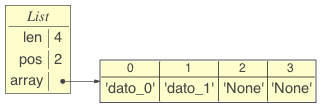
\includegraphics[width=.5\textwidth]{input/05-List-fig/ejemListaConArray}}
\end{ejemplo}

Notar que en todas las primitivas de la definición de una lista, el valor de \cm[black]{pos},  será un entero  entre 0 y \cm[black]{length()-1}. Indicar también  que un array se dimensiona a cierto tamaño y, por tanto, la lista tendrá una cantidad finita de elementos (la del tamaño del array). Un exceso de elementos generaría un error de capacidad. Además, un iterador para una lista no es más que un iterador del array de la estructura de representación.



%%%%%%%%%%%%%%%%%%%%%%%%%%%%%%%%%%%%%%%%%%%%%%%%%%%%%%%%%%%%%%%%%%%%%%%%%%%%%%%%%%%%
%%%%%%%%%%%%%%%%%%%%%%%%%%%%%%%%%%%%%%%%%%%%%%%%%%%%%%%%%%%%%%%%%%%%%%%%%%%%%%%%%%%%

\subsection*{4.C.2 Implementación con  Estructuras Enlazadas}
\addcontentsline{toc}{subsection}{4.C.2. Implementación con Estructuras Enlazadas}
\label{sec:EstructurasEnlazadas}

Las Estructuras Enlazadas son las que cumplen estas condiciones:
\begin{itemize}
\item Representan a colecciones.
\item Constan de nodos (pág \pageref{def:coneptoNodo}).
\item Cada nodo contiene información de interés.
\item Cada nodo contiene referencia a otros nodos.
\item Los nodos se crean cuando son necesario por lo que no tienen por qué almacenarse de forma consecutiva en la memoria.
\end{itemize}


La versión más simple de un nodo es la que consta de un valor y una referencia a otro nodo. La estructura construida con estos nodos se llama \concepto{Estructura Simplemente Enlazada} y es la que usaremos para representar a una lista.

Una \concepto{Lista Simplemente Enlazada} es la representación de una lista que usa una Estructura Simplemente Enlazada:

\hfil
\begin{minipage}{.2\textwidth}
\begin{pyverbatim}[][frame=single]
struct node {
   TD valor;
   node next;
}
\end{pyverbatim}
\end{minipage}


La \key{función de abstracción}:
$
Abst: \mbox{\textbf{node}} \longrightarrow {\cal A}
$
la definiremos como

\centerline{\ttfamily{$Abst($r$) = <$r.valor, r.next.valor, $\ldots$, r.next.\ldots.next.valor$>$}}



Las representaciones legítimas vienen dadas por un predicado,
el \key{invariante de la representación} 
$I: \mbox{\textbf{node}} \longrightarrow \mathbb{B}$, que se define con las siguientes condiciones:
\begin{itemize}
\item Consta de una colección de nodos donde cada uno tiene una referencia a otro nodo (cuyo campo llamaremos \cm[black]{siguiente}/next).

\item Dos nodos diferentes no tienen como referencia \cm[black]{siguiente} el mismo nodo.

\item Se tiene una variable externa que hace referencia a aquel nodo tal que a partir de él se puede recorrer todos los elementos de la lista pasando por la referencia del \cm[black]{siguiente}.
\end{itemize}


\begin{ejemplo}
De esta forma se representará la lista $<dato_0, dato_1, dato_2>$  según una lista simplemente enlazada:

\centerline{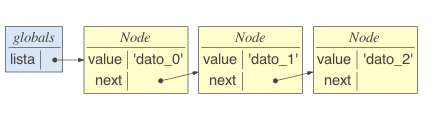
\includegraphics[width=.6\textwidth]{input/05-List-fig/ejemListaSingleLinked}}
\end{ejemplo}

\noindent \textbf{Observaciones:}
\begin{itemize}
\item 
Las estructuras enlazadas, a diferencia del array, no  necesita hacer reservas de posiciones consecutivas de memoria, con lo que la lista puede aumentar mientras que exista memoria suficiente. 

\item 
Los elementos \pyv{Node.value} de la lista se localizan a través de la posición (referencia) del nodo \pyv{Node} que lo contiene. Así pues, \cm[black]{pos} en todas las primitivas debería ser una referencia a un nodo, mientras que en un array la posición es un índice del array.
\end{itemize}



\subsection*{Operaciones básicas en estructuras simplemente enlazadas} \label{subsec:operacionesBasicasSimplemente}
 Las  operaciones que mejor debes entender son
\begin{itemize}
\item Recorrer los nodos
\item Buscar un nodo
\item Añadir un nodo como siguiente de otro.
\item Eliminar el nodo siguiente de otro.
\end{itemize}

\

\noindent \textbf{Recorrer los nodos} se puede expresar de la siguiente forma:
\label{pag:recorrerNodos}

\hfil\begin{minipage}{.38\textwidth}
\begin{pyverbatim}[][frame=single]
actual = primer nodo de la lista
mientras actual is not None:
  trabajar con actual
  actual = actual.next
\end{pyverbatim}
\end{minipage}

Trabajar con actual suele consistir en invocar a alguna función pasando como parámetro \pyv{actual} (p.e. \pyv{print(actual.value)}).
No es necesario recorrer toda la lista. En ocasiones el número de actualizaciones de \pyv{actual} viene dado por el valor \cm[black]{pos} de las primitivas.


\

\noindent \textbf{Buscar un nodo} se puede expresar de la siguiente forma:

\hfil\begin{minipage}{.6\textwidth}
\begin{pyverbatim}[][frame=single]
actual = primer nodo de la lista
mientras actual is not None y actual.value != target:
  actual = actual.next
trabajar con actual
\end{pyverbatim}
\end{minipage}

Este código es el típico código para la función que indica si existe algún valor en la lista (retornando un booleano) y para la función que retorna la posición (o referencia) donde se encuentra el valor encontrado.


\

\noindent \textbf{Añadir un nodo como siguiente de otro} consta de los siguientes pasos:

\begin{enumerate}
\item Tener la referencia del nodo referente.

\hfil\begin{minipage}{.3\textwidth}
\pyv{pos = referencia}
\end{minipage}
\begin{minipage}{.6\textwidth}
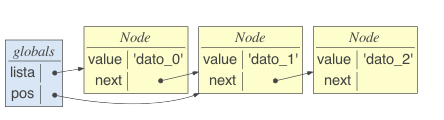
\includegraphics[width=.8\textwidth]{input/05-List-fig/ejemListaSingleLinkedInsert1}
\end{minipage}


\item Crear un nodo que contenga el valor a añadir en la lista.

\hfil\begin{minipage}{.3\textwidth}
\pyv{nuevo_nodo = Node(VALUE)}
\end{minipage}
\begin{minipage}{.6\textwidth}
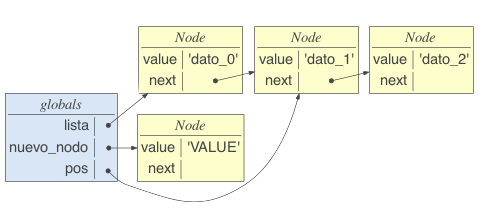
\includegraphics[width=.8\textwidth]{input/05-List-fig/ejemListaSingleLinkedInsert2}
\end{minipage}

\item Enlazar el nuevo nodo con el siguiente del nodo referente.

\hfil\begin{minipage}{.3\textwidth}
\pyv{nuevo_nodo = pos.next}
\end{minipage}
\begin{minipage}{.6\textwidth}
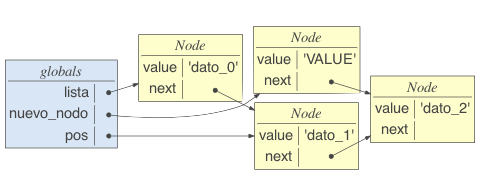
\includegraphics[width=.8\textwidth]{input/05-List-fig/ejemListaSingleLinkedInsert3}
\end{minipage}

\item Enlazar el nodo referente con el nuevo nodo.

\hfil\begin{minipage}{.3\textwidth}
\pyv{pos.next = nuevo_nodo}
\end{minipage}
\begin{minipage}{.6\textwidth}
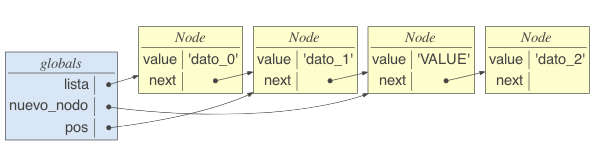
\includegraphics[width=\textwidth]{input/05-List-fig/ejemListaSingleLinkedInsert4}
\end{minipage}

\end{enumerate}


\

\noindent \textbf{Eliminar el nodo siguiente de otro} consta de los siguientes pasos:
\begin{enumerate}
\item Tener la referencia del nodo referente.

\hfil\begin{minipage}{.3\textwidth}
\pyv{pos = referencia}
\end{minipage}
\begin{minipage}{.6\textwidth}
\centerline{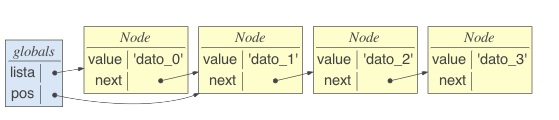
\includegraphics[width=\textwidth]{input/05-List-fig/ejemListaSingleLinkedDeleted1}}
\end{minipage}





\item Enlazar el nodo referente con el nodo siguiente de su nodo siguiente.


\hfil\begin{minipage}{.3\textwidth}
\pyv{borrar = pos.next}\\
\pyv{pos.next = borrar.next}
\end{minipage}
\begin{minipage}{.6\textwidth}
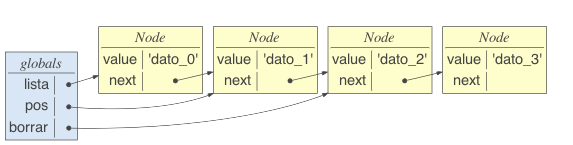
\includegraphics[width=\textwidth]{input/05-List-fig/ejemListaSingleLinkedDeleted2}
\end{minipage}


\item Liberar la memoria del nodo siguiente del nodo referente.

\hfil\begin{minipage}{.3\textwidth}
\pyv{gc.collect()}

En la práctica, esta invocación no se realiza.
\end{minipage}
\begin{minipage}{.6\textwidth}
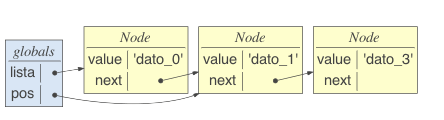
\includegraphics[width=.9\textwidth]{input/05-List-fig/ejemListaSingleLinkedDeleted3}
\end{minipage}

\end{enumerate}

Un punto a tener en cuenta al trabajar con estructuras de datos enlazadas es que con el fin de simplificar la escritura de las funciones, en el sentido de tener que evitar casos especiales en el proceso de inserción y eliminación, es evitar cambiar la referencia de la variable externa al inicio de la estructura. 

Por ejemplo, en un lista simplemente enlazada, si se eliminara el primer elemento de la lista, entonces la referencia de la variable externa tendrá que cambiarse para que apunte al segundo elemento de la lista. De la misma forma, si se quiere añadir un elemento antes del primer elemento de la lista, entonces la referencia de la variable externa tendrá que cambiar al nuevo elemento insertado. 

Una forma de evitar estos casos (aquellos en los que la variable externa cambia su valor de referencia) es considerar la existencia de un nodo intermedio entre la variable externa y el primer término de la lista. Es un nodo que recibe el nombre de \textbf{nodo cabecera} (head) que no contendrá ningún valor y como elemento siguiente hará referencia al primer elemento de la lista, así mismo la variable externa siempre hará referencia al nodo cabecera (y nunca cambiará).

\centerline{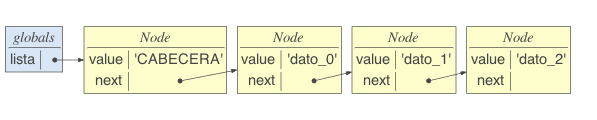
\includegraphics[width=.65\textwidth]{input/05-List-fig/ejemListaSingleLinkedConCabecera}}


Un problema que presenta las listas simplemente enlazadas es que obtener ciertas posiciones para ciertas operaciones puede ser un proceso muy costoso. 
Una de esas situaciones es \textbf{añadir un elemento al final} de la lista. Por ejemplo, si en una lista de $10^6$ elementos se quiere añadir un elemento al final de la misma, será necesario recorrer todos los elementos para poder modificar la referencia del campo siguiente del último nodo. Una forma de resolver este problema es considerar en la estructura una referencia al último nodo:

\hfil
\begin{minipage}{.2\textwidth}
\begin{pyverbatim}[][frame=single]
struct List {
  struct node {
    TD valor;
    node next;
  }
  
  node first
  node last
}
\end{pyverbatim}
\end{minipage}

Otra situación complicada es cuando se necesita recuperar la posición anterior a una posición dada. Por ejemplo, si en una lista de $10^6$ elementos se quiere añadir un elemento en la penúltima posición de la misma, será necesario recorrer los primeros $10^6-1$ elementos de la lista. La situación se agrava si se quisiera recorrer la lista en orden inverso y mostrar sus valores: primero sería necesario recorre $10^6$ elementos, después $10^6-1$, después $10^6-2$, etc. Una forma de solucionar este problema es considerar \textbf{Estructuras Enlazadas con dos enlaces}.

Una \concepto{Lista Doblemente Enlazada} es una representación que usa una Estructura Enlazada con dos Enlaces. El primer enlace hace referencia al elemento siguiente en la lista y el segundo enlace hace referencia al elemento anterior en la lista.

\hfil
\begin{minipage}{.23\textwidth}
\begin{pyverbatim}[][frame=single]
struct node {
   TD valor;
   node next;
   node previous;
}
\end{pyverbatim}
\end{minipage}


\begin{ejemplo}
La lista doblemente enlazada (sin cabecera) para la lista $<dato_0, dato_1, dato_2>$ es:

\centerline{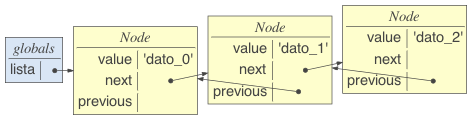
\includegraphics[width=.65\textwidth]{input/05-List-fig/ejemListaDoubleLinked}}
\end{ejemplo}





%%%%%%%%%%%%%%%%%%%%%%%%%%%%%%%%%%%%%%%%%%%%%%%%%%%%%%%%%%%%%%%%%%%%%%%%%%%%%%%%%%%%
%%%%%%%%%%%%%%%%%%%%%%%%%%%%%%%%%%%%%%%%%%%%%%%%%%%%%%%%%%%%%%%%%%%%%%%%%%%%%%%%%%%%

\section*{4.D Búsqueda y Ordenación}
\addcontentsline{toc}{section}{4.D. Búsqueda y Ordenación}

En todas las estructuras de datos que conlleven una colección de datos (p.e. arrays, conjuntos, ficheros, mapas, ...) hay dos tipos de operadores/funciones imprescindibles para el recorrido en la colección de datos y su manipulación: la búsqueda y la ordenación.

\begin{itemize}
\item El objetivo de la búsqueda  es encontrar un dato  concreto. Por ejemplo, en una lista de números naturales localizar el mayor número primo.

\item La ordenación está relacionada con modificar/crear una estructura para que sus elementos se almacenen ordenados según cierto criterio. Es usual que esta estructura sea una lista. Por ejemplo, dada una lista de números naturales crear una nueva lista donde estén ordenarlos de forma creciente.
\end{itemize}


\begin{note}
En lo que sigue, supondremos que la búsqueda y ordenación se hará sobre listas.
También se asume que de la asignatura de \textit{Fundamentos de Programación} se conocen perfectamente los algoritmos de búsqueda secuencial y binaria, así como los algoritmos de ordenación de la burbuja, selección e inserción.
\end{note}

%%%%%%%%%%%%%%%%%%%%%%%%%%%%%%%%%%%%%%%%%%%%%%%%%%%%%%%%%%%%%%%%%%%%%%%%%%%%%%%%%%%%
%%%%%%%%%%%%%%%%%%%%%%%%%%%%%%%%%%%%%%%%%%%%%%%%%%%%%%%%%%%%%%%%%%%%%%%%%%%%%%%%%%%%

\subsection*{4.D.1 Búsqueda}
\addcontentsline{toc}{subsection}{4.D.1. Búsqueda}


Un \concepto{algoritmo de búsqueda} es aquel que está diseñado para localizar un elemento con ciertas propiedades dentro de una estructura de datos. Por ejemplo, encontrar el registro correspondiente a cierta canción en un array de canciones.

Dependiendo de cómo se encuentren ordenados los elementos de la colección, podemos aplicar uno de los dos siguientes algoritmos: 
\begin{itemize}
\item o búsqueda secuencial, cuando los elementos de la colección no están ordenados
\item o búsqueda binaria, para cuando los elementos están ordenados.
\end{itemize}

\noindent Pero  ?`cuándo una lista de objetos esta ordenada? 
\begin{itemize}
\item Una lista {\tt vec} se dice que tiene un orden ascendente si

\centerline{{\tt i$\leq$j} implica que {\tt vec[i]$\leq$vec[j]}} 

\item Una lista {\tt vec} se dice que tiene un orden descendente si

\centerline{{\tt i$\leq$j} implica que {\tt vec[i]$\geq$vec[j]}}

\item Una lista {\tt vec} se dice que está ordenada si presenta un orden ascendente
o un orden descendente 
\end{itemize}


\vspace{0.5cm}
\noindent
El orden puede venir dado (impuesto) o puede que tengas que definirlo tú.
Todo depende del tipo de dato que contenga la lista.
\begin{itemize}
\item Si el tipo de dato de la lista son números, el orden viene dado por el orden de los números tal y como lo conoces.
\item Si la colección es de caracteres, el orden viene dada por la tabla de códigos.
\item Si el conjunto es de valores booleanos, se suele considerar que \cm{true} es mayor que \cm{false}; pero este orden no siempre viene implementado en los lenguajes de programación. Es posible que el orden lo tengas que implementar tú. \cm[red]{Processing} no tienen implementado ningún orden en los booleanos pero para \cm[red]{Python} son números naturales.
\item Si el array es de String, el orden será el lexicográfico. 
\item Si el array es de arrays, tú tendras que definir el orden.
\item Si la colección es de registros, tú tendrás que establecer qué campo o conjuntos de campos son los que establecen que un registro sea posterior que otro.
\end{itemize}


\paragraph*{Búsqueda secuencial.} La búsqueda secuencial se usa cuando los datos no están ordenados. Se puede expresar de la siguiente manera:


\begin{pyverbatim}[][frame=single]
def busqueda_secuencial(lista, dato) -> Optional[int]
  pos = 0  
  for pos in range(len(lista)):
    Si lista[pos].value == dato:
      return pos 
  return None
\end{pyverbatim}


\paragraph*{Búsqueda Binaria.} La búsqueda binaria se usa cuando los datos  están ordenados. Se puede expresar de la siguiente manera, supuesto que la lista ya ha sido ordenada previamente:


\begin{pyverbatim}[][frame=single]
def busqueda_binaria(lista, dato) -> Optional[int]
  size = len(lista)
  inf = 0
  sup = size-1
    
  while inf <= sup:
    pos = ((sup - inf) // 2) + inf // División entera: se trunca la fracción
    if lista[pos].value == dato:
      return pos
    else:
      if dato < lista[pos]:
        sup = pos - 1
      else:
        inf = pos + 1

  return None
\end{pyverbatim}




%%%%%%%%%%%%%%%%%%%%%%%%%%%%%%%%%%%%%%%%%%%%%%%%%%%%%%%%%%%%%%%%%%%%%%%%%%%%%%%%%%%%
%%%%%%%%%%%%%%%%%%%%%%%%%%%%%%%%%%%%%%%%%%%%%%%%%%%%%%%%%%%%%%%%%%%%%%%%%%%%%%%%%%%%

\subsection*{4.D.1 Ordenación}
\addcontentsline{toc}{subsection}{4.D.1. Ordenación}


Un \concepto{algoritmo de ordenación}\footnote{Puede visualizar el funcionamiento de los algoritmos que se muestran en esta sección en \url{https://www.cs.usfca.edu/~galles/visualization/ComparisonSort.html}} u ordenamiento es aquel que está diseñado para ordenar los elementos de una lista. Para esto será necesario aclarar qué se entiende por la expresión \cm{vec[pos1]$<$vec[pos2]}, aspecto que ya se ha comentado. Dicha expresión de comparación deberá interpretarse como una función u operación construida por el programador.



\paragraph*{Ordenación de Burbuja.} La Ordenación de burbuja (Bubble Sort en inglés) funciona revisando cada elemento de la lista que va a ser ordenado con el siguiente, intercambiándolos de posición si están en el orden equivocado y si están en posiciones correctas continúa el proceso con el siguiente elemento. Más concretamente, en cada iteración recorre toda la lista,  desde el inicio de la lista  y hasta el final. En el recorrido compara cada par de elementos adyacentes y si no están en el orden esperado los intercambia de lugar. El proceso continúa hasta que no haya más elementos que necesiten ser comparados. Se puede expresar de la siguiente manera:

\begin{pyverbatim}[][frame=single]
def sort_bubble(vec):
  tam = length(vec)
  do:
    nuevoTam = 0
    for pos in range(1, tam):
      if vec[pos-1] > vec[pos]:
        intercambiar(vec[pos-1], vec[pos])
        nuevoTam = pos
    tam = nuevoTam
  mientras tam != 0
\end{pyverbatim} 


\paragraph*{Ordenación por selección.} 

Imagina que dispones de $n$-valores (todos) distintos en un vector y sabes que están desordenados. ?`Dónde colocarías el elemento más pequeño? ?`y el segundo más pequeño? ?`y el tercero? .... ?`encuentras un patrón? Es fácil, hay que colocar el $k$-ésimo valor más grande en la $k$-ésima posición del array. A partir de esta idea nos planteamos el siguiente algoritmo de ordenación:
\begin{enumerate}
\item Buscar el mínimo elemento de la lista e intercambiarlo con el primero,
\item buscar el siguiente mínimo en el resto de la lista e intercambiarlo con el segundo

...

\item[n.] y así sucesivamente hasta llegar al último.
\end{enumerate}

\noindent Esta secuencia de acciones determinan el siguiente patrón repetitivo:
\begin{enumerate}
\item Buscar el mínimo elemento de la lista que está entre la posición \cm{pos} y el final de la lista (inicialmente \cm{pos=0})
\item Intercambiarlo con el que está entre en la posición \cm{pos}
\item Hacer \cm{pos++}
\end{enumerate}

\noindent El algoritmo se puede expresar así:

\begin{pyverbatim}[][frame=single]
def sort_selection(vec):
  for pos in range(len(vec)):
    pos_minimo = pos
    for siguiente in range(pos+1, tam):     # Busca el valor más pequeño
      if vec[pos_minimo] > vec[siguiente]:  # de entre los siguientes
        pos_minimo = siguiente;
    intercambiar(vec[pos], vec[pos_minimo])     
\end{pyverbatim} 


\paragraph*{Ordenación por inserción.} 

El planteamiento de este algoritmo es el siguiente. Si tuvieses una lista de elementos, para los que sabes que todos los elementos que hay antes de cierta posición \cm{pos-1} sus elementos ya están ordenados ?`cuál es la posición que le corresponde al elemento de la posición \cm{pos} en esa lista? Pues se trataría simplemente de recorrer la lista desde el principio y encontrar {\bf el primer elemento que sea mayor que él} en la lista (si lo hubiera). Si se encontrase en cierta posición \cm{k}, entonces desplazaríamos toda la sublista de las posiciones \cm{[k, pos-1]} a las posiciones \cm{[k+1,pos]}, y el elemento que se encontraba en \cm{pos} se pasaría a la posición \cm{k}. Es decir, insertamos el elemento de la posición \cm{pos} en la posición \cm{k}.

El proceso de inserción también se puede hacer desde el ``último'' elemento de la sublista: Considera una variable \cm{anterior} que represente a las posiciones que se encuentran antes de \cm{pos}, se puede repetir el ciclo de pasar el elemento que está en la posición \cm{anterior} a la posición \cm{anterior+1} (y decrementando en una unidad el valor de \cm{anterior}) mientras que el elemento original que estaba en \cm{pos} {\bf  sea más pequeño} que los elementos determinados por \cm{anterior}. Cuando \cm{anterior} corresponda a una posición cuyo valor  sea mayor que el valor que originalmente estaba en \cm{pos} deja de hacer los intercambios, en cuyo caso dejará un ``hueco'' que es aprovechado para insertar el valor que se encontraba en \cm{pos}. El algoritmo se puede expresar así:

\begin{pyverbatim}[][frame=single]
def sort_insertion(vec)
  for pos in range(1, len(vec)):
    valor = vec[pos]
    anterior = pos - 1
    while anterior >= 0 and vec[anterior] > valor:
      vec[anterior+1] = vec[anterior]
      anterior = anterior - 1
    vec[anterior + 1] = valor      
\end{pyverbatim}





\paragraph{Ordenación por casilleros.} 
Todos los algoritmos anteriores son algoritmos de orden $O(n^2)$.
Esto quiere decir que el número de operaciones que tiene que hacer, en el peor de los casos, es proporcional a $n^2$ para $n$ igual al número de datos a ordenar.
En otras palabras, en el peor de los casos, el ordenador que quiera ordenar mil objetos tendrá que realizar un número de operaciones proporcional a  $(10^3)^2=10^6$.
Teniendo en cuenta que hay algoritmos en el mundo de la informática muchísimo más complicados y que prácticamente nunca acaban, se podría pensar que estos algoritmo ``no están nada mal''; pero si te digo que hay muchos algoritmos de ordenación cuya complejidad computacional es mucho menor (son del orden $O(n\; log(n))$ y $O(n)$) y que los peores algoritmos de ordenación son los de orden $O(n^2)$ ...  tengo que decirte que se te han explicado los algoritmos más sencillos pero también los más ineficientes si tienes que ordenar muchos, muchos datos.

Para mejorar la eficiencia de los algoritmos anteriores, te mostramos un algoritmo muy simple de orden $O(n)$, que es la ordenación por casilleros (o cubos - bucket sort o bin sort, en inglés).

El algoritmo se divide en dos partes.

\begin{enumerate}
\item En la primera, se considerar una serie de casilleros o cubos en los que solo debes introducir los elementos de la lista a ordenar que cumpla las condiciones del casillero. Las condiciones entre los casilleros deben ser excluyentes entre sí, para evitar que un elemento pueda ser clasificado en dos cubos distintos.  

Por ejemplo, si vas a ordenar un lista de números naturales $\{29,25,3,49,9,37,21,43\}$  puedes definir el cubo $k$ como el que contiene los números comprendidos entre $k\times 10$ y $(k+1)\times 10 -1$. Con lo que los cubos quedan como $C_0=\{3,9\}$, $C_2=\{29,25,21\}$, $C_3=\{37\}$ y $C_4=\{49,43\}$

\item En la segunda parte se ordenan los elementos de cada uno de esos casilleros con otro algoritmo de ordenación (que podría incluso ser distinto según el casillero) o se aplica recursivamente este algoritmo para obtener casilleros con menos elementos. 

Por ejemplo, tras ordenar los cubos anteriores se quedan como $C_0=\{3,9\}$, $C_2=\{21, 25, 29\}$, $C_3=\{37\}$ y $C_4=\{43,49\}$. Y el orden de la lista final queda como ``la concatenación'' de los elementos de cada uno de los cubos: 
$\{3,9, 21, 25, 29, 37,43,49\}$.
\end{enumerate}

El algoritmo puede expresarse en 4 pasos:
\begin{enumerate}
\item Crear una colección de casilleros vacíos, que ya está ``ordenados'' entre sí.
\item Colocar cada elemento a ordenar de la lista en un único casillero.
\item Ordenar los elementos de cada casillero según el algoritmo que se considere más adecuado.
\item Devolver los elementos de cada casillero ``concatenados''.
\end{enumerate}



El algoritmo se puede expresar así:
\begin{pyverbatim}[][frame=single]
def sort_basket(vec)
  # Primer paso: crea los casilleros de forma adecuada
  cubos = new Coleccion (nCubos) 

  # Segundo paso: introduce cada elemento en un casillero
  for pos in range(len(vec)):
    insertar(vec[pos], cubos)

  # Tercer paso: ordena los casilleros
  for pos in range(nCubos):
    cubos[pos].sort()
    
  # Cuarto paso: devuelve la solución
  return concatena(cubos)
\end{pyverbatim}



\paragraph{Merge Sort (Ordenación por mezcla).}  \label{sec:mergeSort}
Este algoritmo recursivo se basa en una idea muy sencilla. Para ordenar una lista basta ordenar la primera mitad lo que nos da una lista1 y ordenar la segunda mitad lo que nos da una lista2.
Entonces basta recorrer uno a uno los elementos de lista1 y compararlos con los elementos de lista2. Si el elemento actual de lista1 es más pequeño se añade al resultado y en otro caso se añade el elemento actual de lista2.

Existen dos versiones de este algoritmo. Se muestra una de ellas copiada de \href{https://en.wikipedia.org/wiki/Merge_sort#:~:text=In\%20computer\%20science\%2C\%20merge\%20sort,in\%20the\%20input\%20and\%20output.}{Wikipedia}. Si quiere conocer la segunda versión consulte el enlace anterior.

\begin{pyverbatim}[][frame=single]
function merge_sort(list m)
    // Base case. A list of zero or one elements is sorted, by definition.
    if length of m <= 1 then
        return m

    // Recursive case. First, divide the list into equal-sized sublists
    // consisting of the first half and second half of the list.
    // This assumes lists start at index 0.
    var left := empty list
    var right := empty list
    for each x with index i in m do
        if i < (length of m)/2 then
            add x to left
        else
            add x to right

    // Recursively sort both sublists.
    left := merge_sort(left)
    right := merge_sort(right)

    // Then merge the now-sorted sublists.
    return merge(left, right)
\end{pyverbatim}

\begin{pyverbatim}[][frame=single]
function merge(left, right)
    var result := empty list

    while left is not empty and right is not empty do
        if first(left) <= first(right) then
            append first(left) to result
            left := rest(left)
        else
            append first(right) to result
            right := rest(right)

    // Either left or right may have elements left; consume them.
    // (Only one of the following loops will actually be entered.)
    while left is not empty do
        append first(left) to result
        left := rest(left)
    while right is not empty do
        append first(right) to result
        right := rest(right)
    return result
\end{pyverbatim}


\


\


\centerline{\Large \bf Ejercicios}



\formatoEjercicio
 


%%%%%%%%%%%%%%%%%%%%%%%%%%%%%%%%%%%%%%%%%%%%%%%%%% 
\separacion
\section{Listas con Array1D} 
\objetivo{2}{-}{Implementar TDA List como Array}

Usa la definición del TDA List de esta sesión para implementarlo
en \cm[red]{Python} usando para su implementación el TDA Array1D de la sesión anterior.
Llama a tu fichero \cm[black]{ListArray.py} y a la clase \cm[black]{List}.

Para su implementación usa la siguiente estructura\footnote{Aquí usaremos el identificador \cm[blue]{Lista} para evitar problemas con  \cm[blue]{List} de \pyv{typing} de Python}:

\hfil
\begin{minipage}{.43\textwidth}
\begin{pyverbatim}[][frame=single]
class Lista: 
   _lista : Array1D # Array de valores
   _pos: int        # Posición 
\end{pyverbatim}
\end{minipage}

\noindent donde \pyv{_lista} será de tipo \cm[black]{Array1D} de cierto tamaño $n$ fijo y 
\pyv{pos} indica la posición donde se almacenará el siguiente elemento a añadir en el array \pyv{_lista}. Inicialmente \pyv{pos} valdrá 0 (es decir, el primer elemento que se añada en el array será en la posición de índice 0). El  array irá cambiando en tiempo de ejecución de acuerdo a los siguientes criterios:
\begin{itemize}
\item Si se añade un nuevo elemento sin especificar su posición y quedan posiciones libres, el dato se almacenará en la posición \pyv{pos}. Pero si se especificara su posición, entonces todos los elementos desde esa posición hasta el final incrementará su posición en una unidad.
En cualquiera de los dos casos se incrementará \pyv{pos} en una unidad. Así, \pyv{pos} se incrementa conforme se vayan añadiendo elementos.
\item Si se añade un nuevo elemento pero todas las posiciones están ocupadas, entonces crea un nuevo array con el doble de capacidad, copia los elementos existentes y añade el nuevo elemento teniendo en cuenta el punto anterior. Después descarta el array usado hasta el momento para usar el que tiene doble capacidad.
\item Si se elimina un elemento de una posición, desplaza todos los elementos 
que se encuentran en las posiciones siguientes a una posición anterior para que 
no queden huecos libres ``al final''. Decrementa \pyv{pos} en una unidad.
\item Si queda un porcentaje $A$ de posiciones libres (p.e. $A=50\%$), entonces
se creará un nuevo array con un porcentaje $B$ de posiciones (p.e. $B=75\%$) y se copiará en él los elementos existentes. El nuevo array nunca tendrá una capacidad inferior al valor $n$ fijo. Después descarta el array usado hasta el momento para usar el que tiene dos tercios de capacidad.
\end{itemize}

Observa que si se trabajara con Array1D de forma estricta (el número de posiciones es siempre igual al número de elementos de la lista), entonces sería necesario crear un array con una dimensión más (si se va a añadir un elemento) o una dimensión menos (si se va a borrar un elemento), copiar los elementos restantes al nuevo array y descartar el array inicial. Desde una perspectiva computacional el coste para usar esta estructura es excesivo (imagina que trabajaras con millones de datos). Por ello, como alternativa, se trabaja con la estructura indicada y que viene de forma nativa en muchos lenguajes de programación.

Ya que se implementará esta estructura en \cm[red]{Python}, los datos se pueden acceder por índice (notación de array) y no por método (notación punto de POO). Para ello implementa los métodos mágicos \cm{\_\_getitem\_\_()} y \cm{\_\_setitem\_\_()}.




% - - - - - - - - - - - - - - - - - - - - - - - - - - - - - - - - - - - - - - - - - - - -

%\input ejercicios/05-Funciones/triplaPitagoricaSol.tex


%%%%%%%%%%%%%%%%%%%%%%%%%%%%%%%%%%%%%%%%%%%%%%%%%% 
\separacion
\section{Lista Simplemente Enlazada} 
\objetivo{2}{-}{Implementar TDA List con Nodos}

Usa la definición del TDA List de esta sesión e implementala
en \cm[red]{Python} usando una estructura simplemente enlazada.
Llama a tu fichero \cm[black]{ListSimpleRefLink.py} y a la clase \cm[black]{List}.


Recuerda que en esta implementación, el valor del parámetro \cm[black]{pos} en todas las primitivas debería ser una referencia a un nodo.



%%%%%%%%%%%%%%%%%%%%%%%%%%%%%%%%%%%%%%%%%%%%%%%%%% 
\separacion
\section{Lista Simplemente Enlazada con Índices} \label{sec:listasimplementeenlazada}
\objetivo{2}{B}{Implementar TDA List con índices y nodos}

En los dos ejercicios anteriores se han implementado dos formas de trabajar con listas: una con índices (arrays) y otra con referencias (nodos). También sabemos que si se usa un TDA Lista nuestro programa debe diseñarse e implementarse independientemente del tipo de implementación del TDA. Por tanto, necesitamos que los valores \cm[black]{pos} sean del mismo tipo en ambas implementaciones de la lista. 

Queremos que \cm[black]{pos} sea un entero en cualquier implementación. En un array se corresponderá con uno de los índices del array y en una estructura enlazada nos indicará el número de veces que tendremos que actualizar las referencias de los nodos.

Utiliza el siguiente esquema para implementar una lista simplemente enlazada usando un entero para acceder a los nodos. Recuerda implementar los métodos mágicos \cm{\_\_getitem\_\_()} y \cm{\_\_setitem\_\_()}.


\begin{pyverbatim}[][frame=single]
class Lista:
    class __Node:
        __slots__ = '_value', '_next'
        _value: object
        _next: Optional['Node']
        
        ....

    __slots__ = '_head', '_len'
    _head: Node
    _len: int

    def __get_node(self, pos: int) -> __Node:
        if pos == -1 or self.empty():
            return self._head

        assert 0 <= pos < len(self), "Posición fuera de límites"
        node = self._head.next
        for i in range(pos): 
            node = node.next
        return node
\end{pyverbatim}
        
Observa que se usa una clase interna que es invisible fuera de la clase (se usa dos líneas bajas antes del nombre de la clase). Observa también que esta implementación del TDA Lista usa un nodo cabecera.



% - - - - - - - - - - - - - - - - - - - - - - - - - - - - - - - - - - - - - - - - - - - -

%\input ejercicios/05-Funciones/AleatoriosSol.tex



%%%%%%%%%%%%%%%%%%%%%%%%%%%%%%%%%%%%%%%%%%%%%%%%%% 
\separacion
\section{Lista Doblemente Enlazada} 
\objetivo{2}{-}{Implementar TDA List con Nodos}

Usa la definición del TDA List de esta sesión para implementarlo
en \cm[red]{Python} usando para su implementación una estructura doblemente enlazada.
Llama a tu fichero \cm[black]{ListDoubleLink.py} y a la clase \cm[black]{List}.

% - - - - - - - - - - - - - - - - - - - - - - - - - - - - - - - - - - - - - - - - - - - -

%\input ejercicios/05-Funciones/AleatoriosSol.tex





%%%%%%%%%%%%%%%%%%%%%%%%%%%%%%%%%%%%%%%%%%%%%%%%%% 
\separacion
\section{Módulo de Búsqueda} \label{sec:moduloBusqueda}
\objetivo{1}{B}{Implementar algoritmos de búsqueda}

Crea el módulo \directory{Searching > SearchingList.py}
e implementa en él los dos algoritmos de búsqueda (secuencial y binaria)
trabajando con las listas de Python. 

Cuando veas que funciona correctamente, adapta las funciones para que sean métodos de las implementaciones que hayas hecho del TDA Lista.

Es decir, si tienes la función \pyv{def search_secuencial()} modifícala para que sea el método  \pyv{def search_secuencial(self)}, que deberás añadir al tipo Lista que has implementado en la sesión anterior.



% - - - - - - - - - - - - - - - - - - - - - - - - - - - - - - - - - - - - - - - - - - - -

%\input ejercicios/05-Funciones/AleatoriosSol.tex



%%%%%%%%%%%%%%%%%%%%%%%%%%%%%%%%%%%%%%%%%%%%%%%%%% 
\separacion
\section{Módulo de Ordenación} \label{sec:moduloOrdenacion}
\objetivo{2}{B}{Implementar algoritmos de ordenación}

Implementa un módulo con distintas técnicas de ordenación de listas. 
Deberá contener, al menos, la ordenación por casilleros y la ordenación por mezcla.
Este módulo lo aplicaremos en la siguiente sesión para aplicar técnicas de búsqueda en espacio de estados que es la forma más general de resolver problemas en Inteligencia Artificial. 

\begin{itemize}
\item Llama a tu fichero \cm[black]{Sort} y a las funciones las llamas \cm[black]{sort\_busket()} y \cm[black]{sort\_merge()}. Ambas funciones tendrán como parámetro de entrada una lista de tipo \pyv{list} de Python - ver página  \pageref{sec:mergeSort}.

Opcionalmente añade las siguientes funciones: \cm[black]{sort\_bubble()}, \cm[black]{sort\_selection()}, \cm[black]{sort\_insertion()}.


\item Implementa el método \cm{def sort(self, method)} como una primitiva más del tipo lista. El parámetro \cm{method} indicará la función a aplicar para la ordenación.
\end{itemize}

% - - - - - - - - - - - - - - - - - - - - - - - - - - - - - - - - - - - - - - - - - - - -

%\input ejercicios/05-Funciones/AleatoriosSol.tex



%%%%%%%%%%%%%%%%%%%%%%%%%%%%%%%%%%%%%%%%%%%%%%%%%% 
\separacion
\section{Ordenar a los alumnos} 
\objetivo{1}{B}{Aplicación de los algoritmos de ordenación. Diccionarios}

En el contexto del Ejercicio \ref{sec:cursosDeTitulo} crea la clase \cm[black]{Acta}. El acta de una asignatura es un documento que consta de una lista donde, en cada fila, figura un alumno junto con la calificación obtenida. Para este ejercicio se supondrá que todos los alumnos tienen una calificación numérica real en el intervalo $[0,10]$ y con un valor decimal. Se pide:

\begin{itemize}
\item 
Crea un conjunto de no menos de 10 alumnos. 
No es importante que los datos de los alumnos tengan sentido, lo importante es que se distingan. Puedes usar un bucle \cm{for} para acelerar el proceso.

\item
Construye entonces un acta con esos alumnos y asigna a cada uno una nota aleatoria.
Recurre al módulo \url{https://docs.python.org/es/3/library/random.html}

\item Ordena a los alumnos del acta de acuerdo a sus calificaciones. 

Mira los métodos mágicos de comparación \pyv{__cmp__()}, \pyv{__lt__()}, \pyv{__qt__()}, ....
A efectos de depuración, necesitarás que todos los alumnos tengan siempre la misma calificación ``aleatoria''  en cada ejecución. Para conseguir que en cada ejecución siempre se generan los mismos números aleatorios usa siempre la misma semilla, p.e. \cm{seed(0)}.

\item Construye un diccionario que indique cuántos alumnos han suspendido ($nota < 5$), han aprobado ($5\leq nota < 7$), tienen notable ($7\leq nota < 9$) o son de sobresaliente ($nota \geq 9$).

El diccionario lo puedes construir usando \cm{dict()} de \cm[red]{Python} o \cm[black]{Map()} del Ejercicio \ref{sec:TDAMap}.
\end{itemize}


% - - - - - - - - - - - - - - - - - - - - - - - - - - - - - - - - - - - - - - - - - - - -

%\input ejercicios/05-Funciones/AleatoriosSol.tex


\separacion


